\section*{Class Hierarchy}{
\thispagestyle{empty}
\markboth{Class Hierarchy}{Class Hierarchy}
\addcontentsline{toc}{section}{Class Hierarchy}

\begin{figure}[!hbp]
	\centering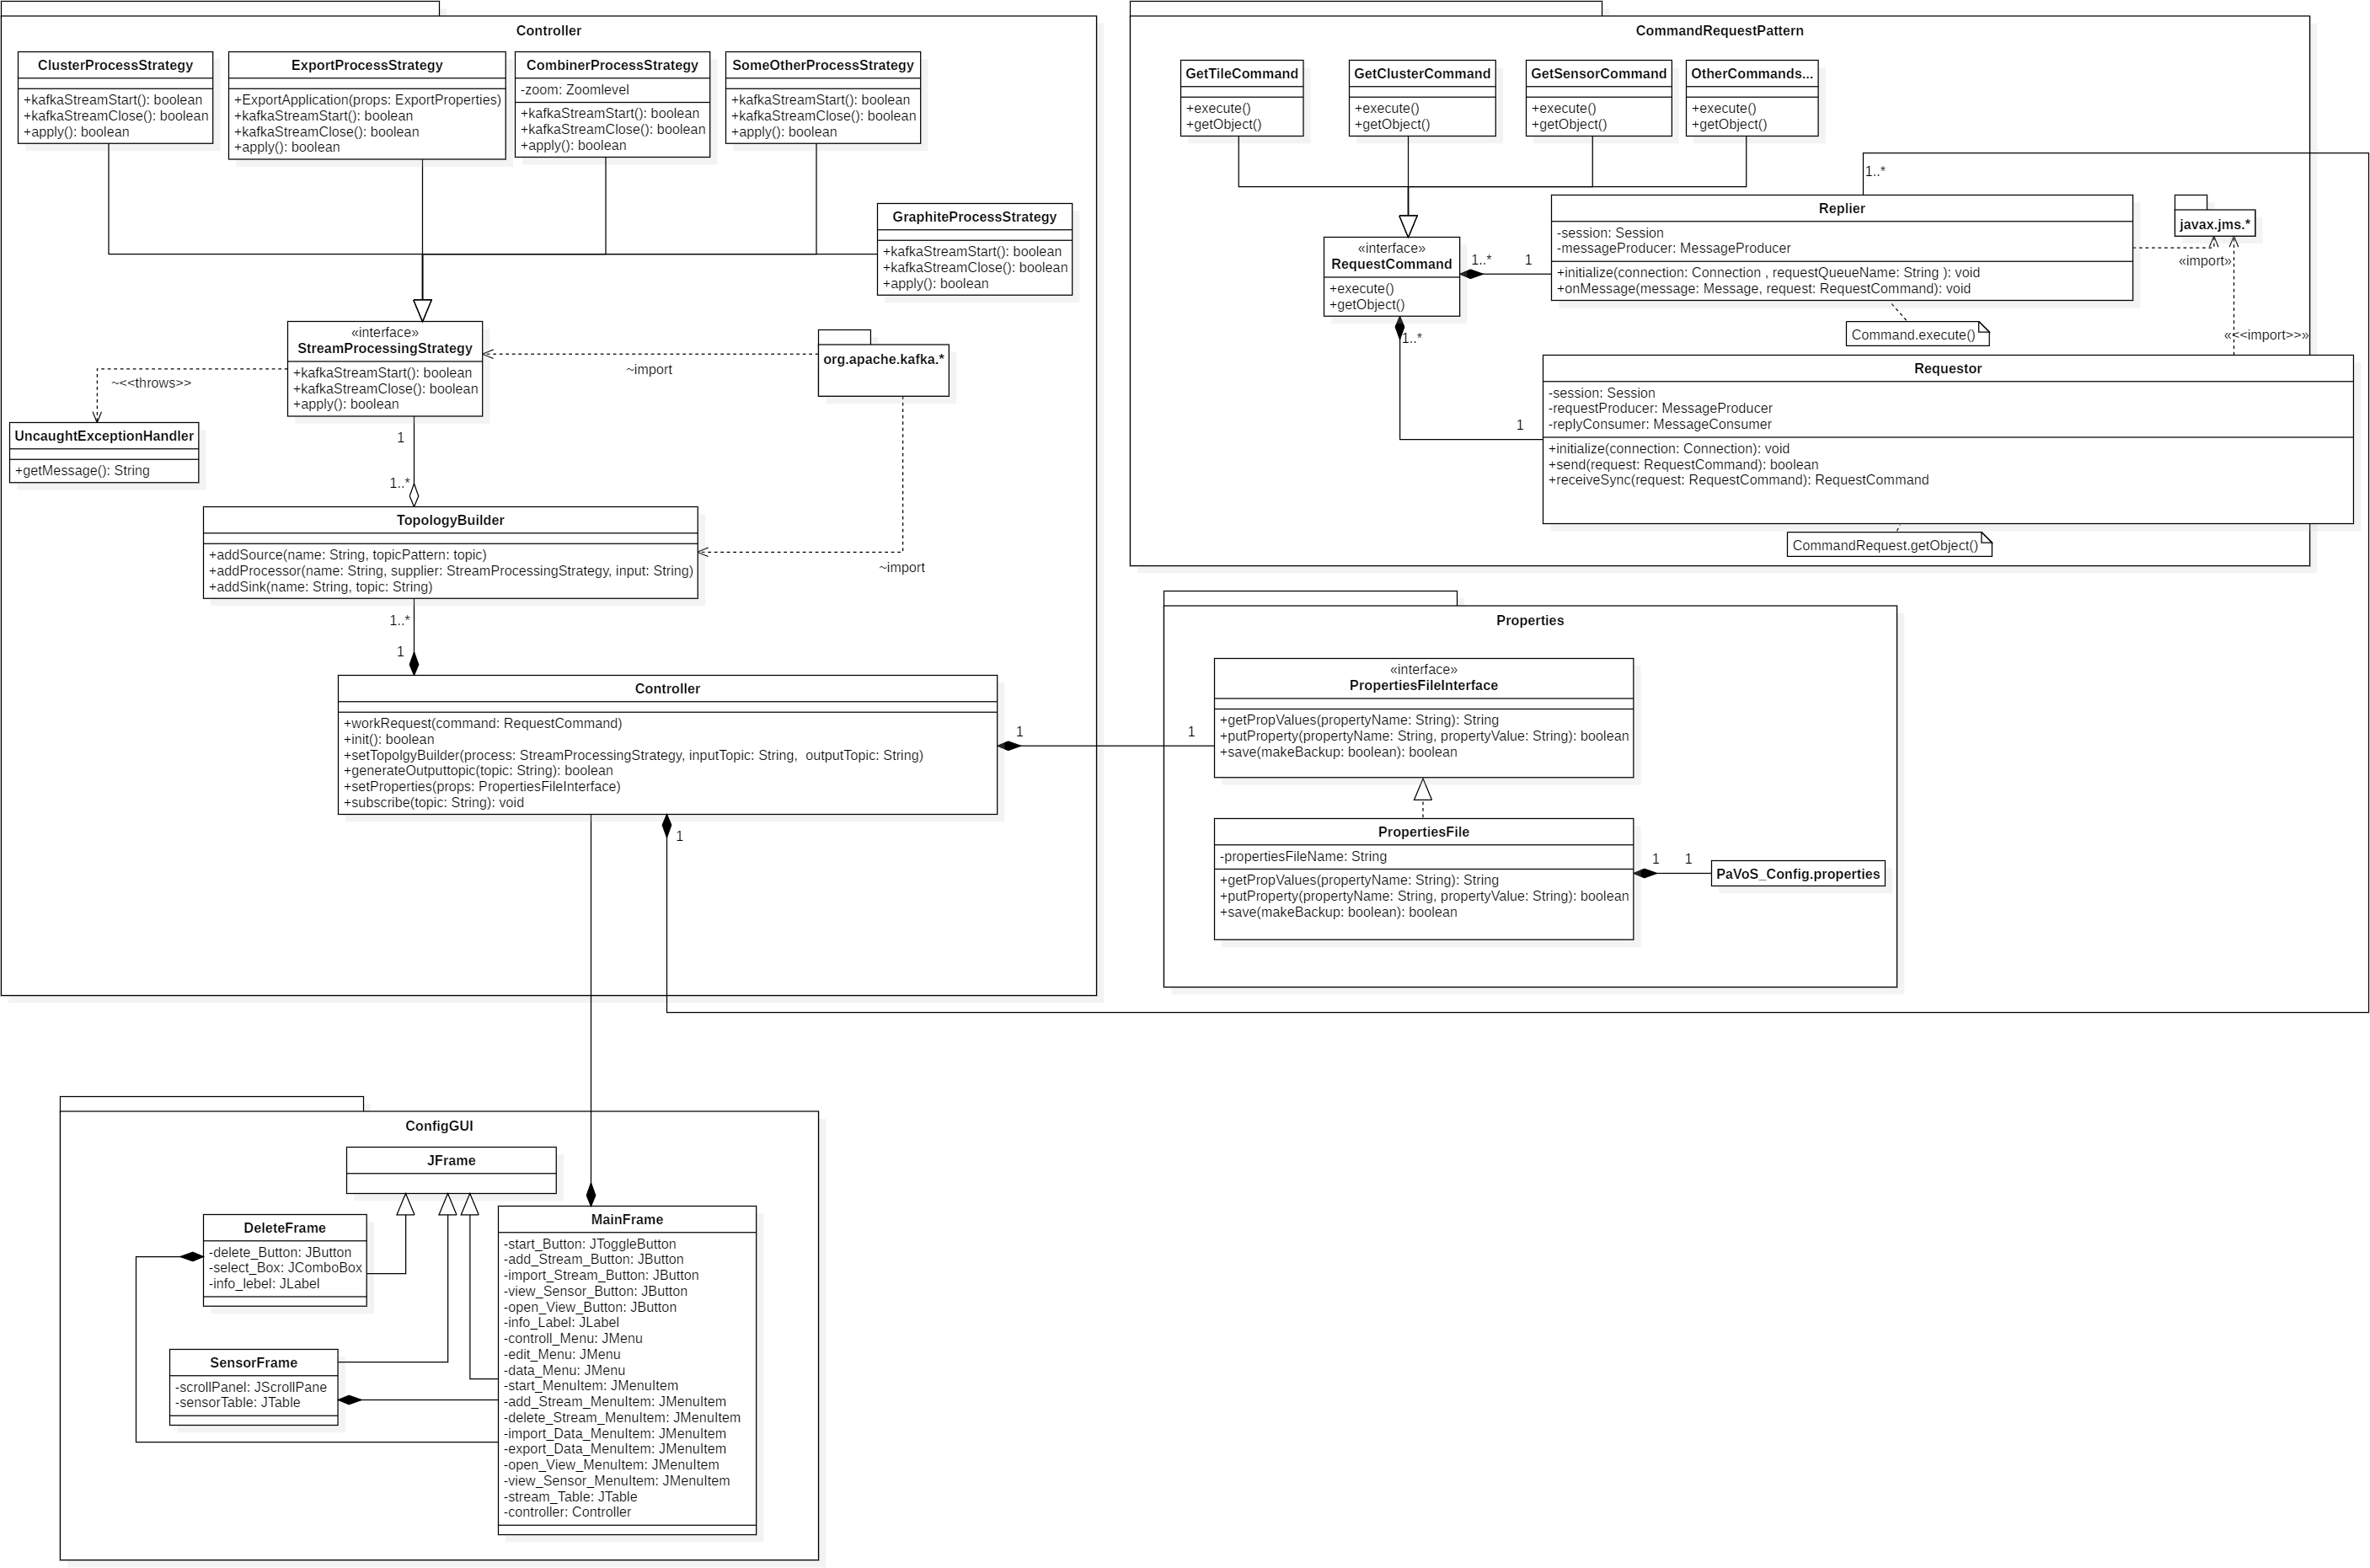
\includegraphics[width=0.8\linewidth]{images/core/CoreClassDiagram}
\end{figure}

\subsection*{Classes}
{\raggedright
\hspace{0.0cm} $\bullet$ java.lang.Object {\tiny \refdefined{java.lang.Object}} \\
\hspace{1.0cm} $\bullet$ CommandRequestPattern.GetClusterCommand {\tiny \refdefined{CommandRequestPattern.GetClusterCommand}} \\
\hspace{1.0cm} $\bullet$ CommandRequestPattern.GetSensorCommand {\tiny \refdefined{CommandRequestPattern.GetSensorCommand}} \\
\hspace{1.0cm} $\bullet$ CommandRequestPattern.GetTileCommand {\tiny \refdefined{CommandRequestPattern.GetTileCommand}} \\
\hspace{1.0cm} $\bullet$ CommandRequestPattern.Replier {\tiny \refdefined{CommandRequestPattern.Replier}} \\
\hspace{1.0cm} $\bullet$ CommandRequestPattern.Requestor {\tiny \refdefined{CommandRequestPattern.Requestor}} \\
\hspace{1.0cm} $\bullet$ ConfigGUI.JFrame {\tiny \refdefined{ConfigGUI.JFrame}} \\
\hspace{2.0cm} $\bullet$ ConfigGUI.DeleteFrame {\tiny \refdefined{ConfigGUI.DeleteFrame}} \\
\hspace{2.0cm} $\bullet$ ConfigGUI.MainFrame {\tiny \refdefined{ConfigGUI.MainFrame}} \\
\hspace{2.0cm} $\bullet$ ConfigGUI.SensorFrame {\tiny \refdefined{ConfigGUI.SensorFrame}} \\
\hspace{1.0cm} $\bullet$ Controller.ClusterProcessStrategy {\tiny \refdefined{Controller.ClusterProcessStrategy}} \\
\hspace{1.0cm} $\bullet$ Controller.CombinerProcessStrategy {\tiny \refdefined{Controller.CombinerProcessStrategy}} \\
\hspace{1.0cm} $\bullet$ Controller.Controller {\tiny \refdefined{Controller.Controller}} \\
\hspace{1.0cm} $\bullet$ Controller.ExportProcessStrategy {\tiny \refdefined{Controller.ExportProcessStrategy}} \\
\hspace{1.0cm} $\bullet$ Controller.GraphiteProcessStrategy {\tiny \refdefined{Controller.GraphiteProcessStrategy}} \\
\hspace{1.0cm} $\bullet$ Controller.TopologyBuilder {\tiny \refdefined{Controller.TopologyBuilder}} \\
\hspace{1.0cm} $\bullet$ Controller.UncaughtExceptionHandler {\tiny \refdefined{Controller.UncaughtExceptionHandler}} \\
\hspace{1.0cm} $\bullet$ Properties.PropertiesFile {\tiny \refdefined{Properties.PropertiesFile}} \\
}
\subsection*{Interfaces}
\hspace{0.0cm} $\bullet$ CommandRequestPattern.RequestCommand {\tiny \refdefined{CommandRequestPattern.RequestCommand}} \\
\hspace{0.0cm} $\bullet$ CommandRequestPattern.StreamProcessingStrategy {\tiny \refdefined{CommandRequestPattern.StreamProcessingStrategy}} \\
\hspace{0.0cm} $\bullet$ Properties.PropertiesFileInterface {\tiny \refdefined{Properties.PropertiesFileInterface}} \\
}
\section{Package CommandRequestPattern}{
\label{CommandRequestPattern}\hypertarget{CommandRequestPattern}{}
\hskip -.05in
\hbox to \hsize{\textit{ Package Contents\hfil Page}}
\vskip .13in
\hbox{{\bf  Interfaces}}
\entityintro{RequestCommand}{CommandRequestPattern.RequestCommand}{All CommandsRequest implements this Interface.}
\entityintro{StreamProcessingStrategy}{CommandRequestPattern.StreamProcessingStrategy}{This Class is a Interface for the Stream Builder Applications which genereates an Output topic to provides data transformations.}
\vskip .13in
\hbox{{\bf  Classes}}
\entityintro{GetClusterCommand}{CommandRequestPattern.GetClusterCommand}{This Command request a Cluster in the System.}
\entityintro{GetSensorCommand}{CommandRequestPattern.GetSensorCommand}{This Command request a Sensor in the System.}
\entityintro{GetTileCommand}{CommandRequestPattern.GetTileCommand}{This Command request a Tile in the System.}
\entityintro{Replier}{CommandRequestPattern.Replier}{This Class handels the Requests and Replies to them}
\entityintro{Requestor}{CommandRequestPattern.Requestor}{The Implemente this class and request something to the System and a Replier answer to it.}
\vskip .1in
\vskip .1in
\subsection{\label{CommandRequestPattern.RequestCommand}Interface RequestCommand}{
\hypertarget{CommandRequestPattern.RequestCommand}{}\vskip .1in 
All CommandsRequest implements this Interface. CommandRequest are sendet form the View to request something out of the System.\vskip .1in
\begin{figure}[!hbp]
	\centering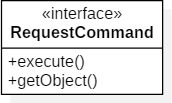
\includegraphics[width=0.2\linewidth]{images/core/classes/RequestCommand}
\end{figure} 
\subsubsection{Declaration}{
\begin{lstlisting}[frame=none]
public interface RequestCommand
\end{lstlisting}
\subsubsection{All known subinterfaces}{GetTileCommand\small{\refdefined{CommandRequestPattern.GetTileCommand}}, GetSensorCommand\small{\refdefined{CommandRequestPattern.GetSensorCommand}}, GetClusterCommand\small{\refdefined{CommandRequestPattern.GetClusterCommand}}}
\subsubsection{All classes known to implement interface}{GetTileCommand\small{\refdefined{CommandRequestPattern.GetTileCommand}}, GetSensorCommand\small{\refdefined{CommandRequestPattern.GetSensorCommand}}, GetClusterCommand\small{\refdefined{CommandRequestPattern.GetClusterCommand}}}
\subsubsection{Method summary}{
\begin{verse}
\hyperlink{CommandRequestPattern.RequestCommand.execute()}{{\bf execute()}} This is the Execution form the requested Command\\
\hyperlink{CommandRequestPattern.RequestCommand.getObject()}{{\bf getObject()}} This Method Return the Requested Object\\
\end{verse}
}
\subsubsection{Methods}{
\vskip -2em
\begin{itemize}
\item{ 
\index{execute()}
\hypertarget{CommandRequestPattern.RequestCommand.execute()}{{\bf  execute}\\}
\begin{lstlisting}[frame=none]
void execute()\end{lstlisting} %end signature
\begin{itemize}
\item{
{\bf  Description}

This is the Execution form the requested Command
}
\end{itemize}
}%end item
\item{ 
\index{getObject()}
\hypertarget{CommandRequestPattern.RequestCommand.getObject()}{{\bf  getObject}\\}
\begin{lstlisting}[frame=none]
void getObject()\end{lstlisting} %end signature
\begin{itemize}
\item{
{\bf  Description}

This Method Return the Requested Object
}
\end{itemize}
}%end item
\end{itemize}
}
}
\subsection{\label{CommandRequestPattern.StreamProcessingStrategy}Interface StreamProcessingStrategy}{
\hypertarget{CommandRequestPattern.StreamProcessingStrategy}{}\vskip .1in 
This Class is a Interface for the Stream Builder Applications which genereates an Output topic to provides data transformations. The ProcessingApplication will use Kafka DSL API to process the data.\vskip .1in 
\begin{figure}[!hbp]
	\centering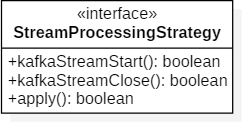
\includegraphics[width=0.2\linewidth]{images/core/classes/StreamProcessingStrategy}
\end{figure} 
\subsubsection{Declaration}{
\begin{lstlisting}[frame=none]
public interface StreamProcessingStrategy
\end{lstlisting}
\subsubsection{Method summary}{
\begin{verse}
\hyperlink{CommandRequestPattern.StreamProcessingStrategy.apply()}{{\bf apply()}} This Methode definite the Process of the Application.\\
\hyperlink{CommandRequestPattern.StreamProcessingStrategy.kafkaStreamClose()}{{\bf kafkaStreamClose()}} This Method is used to explicitly close the Kafka Stream thread.\\
\hyperlink{CommandRequestPattern.StreamProcessingStrategy.kafkaStreamStart()}{{\bf kafkaStreamStart()}} This Method is used to explicitly start the Kafka Stream thread.\\
\end{verse}
}
\subsubsection{Methods}{
\vskip -2em
\begin{itemize}
\item{ 
\index{apply()}
\hypertarget{CommandRequestPattern.StreamProcessingStrategy.apply()}{{\bf  apply}\\}
\begin{lstlisting}[frame=none]
boolean apply()\end{lstlisting} %end signature
\begin{itemize}
\item{
{\bf  Description}

This Methode definite the Process of the Application. What Application does specificly.
}
\item{{\bf  Returns} -- 
true if the Process got Successfully worked 
}%end item
\end{itemize}
}%end item
\item{ 
\index{kafkaStreamClose()}
\hypertarget{CommandRequestPattern.StreamProcessingStrategy.kafkaStreamClose()}{{\bf  kafkaStreamClose}\\}
\begin{lstlisting}[frame=none]
boolean kafkaStreamClose()\end{lstlisting} %end signature
\begin{itemize}
\item{
{\bf  Description}

This Method is used to explicitly close the Kafka Stream thread. So that the Processing stops.
}
\item{{\bf  Returns} -- 
true if the Kafka Stream closed, false otherwise 
}%end item
\end{itemize}
}%end item
\item{ 
\index{kafkaStreamStart()}
\hypertarget{CommandRequestPattern.StreamProcessingStrategy.kafkaStreamStart()}{{\bf  kafkaStreamStart}\\}
\begin{lstlisting}[frame=none]
boolean kafkaStreamStart()\end{lstlisting} %end signature
\begin{itemize}
\item{
{\bf  Description}

This Method is used to explicitly start the Kafka Stream thread. So that theProcessing need to get started.
}
\item{{\bf  Returns} -- 
true if the Kafka Stream Started false otherwise 
}%end item
\end{itemize}
}%end item
\end{itemize}
}
}
\subsection{\label{CommandRequestPattern.GetClusterCommand}Class GetClusterCommand}{
\hypertarget{CommandRequestPattern.GetClusterCommand}{}\vskip .1in 
This Command request a Cluster in the System.\vskip .1in 
\begin{figure}[!hbp]
	\centering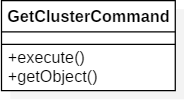
\includegraphics[width=0.2\linewidth]{images/core/classes/GetClusterCommand}
\end{figure} 
\subsubsection{Declaration}{
\begin{lstlisting}[frame=none]
public class GetClusterCommand
 extends java.lang.Object implements RequestCommand\end{lstlisting}
\subsubsection{Constructor summary}{
\begin{verse}
\hyperlink{CommandRequestPattern.GetClusterCommand()}{{\bf GetClusterCommand()}} Default constructor\\
\end{verse}
}
\subsubsection{Method summary}{
\begin{verse}
\hyperlink{CommandRequestPattern.GetClusterCommand.execute()}{{\bf execute()}} This is the Execution form the requested Command.\\
\hyperlink{CommandRequestPattern.GetClusterCommand.getObject()}{{\bf getObject()}} This Method Return the Requested Cluster as a KStream\\
\end{verse}
}
\subsubsection{Constructors}{
\vskip -2em
\begin{itemize}
\item{ 
\index{GetClusterCommand()}
\hypertarget{CommandRequestPattern.GetClusterCommand()}{{\bf  GetClusterCommand}\\}
\begin{lstlisting}[frame=none]
public GetClusterCommand()\end{lstlisting} %end signature
\begin{itemize}
\item{
{\bf  Description}

Default constructor
}
\end{itemize}
}%end item
\end{itemize}
}
\subsubsection{Methods}{
\vskip -2em
\begin{itemize}
\item{ 
\index{execute()}
\hypertarget{CommandRequestPattern.GetClusterCommand.execute()}{{\bf  execute}\\}
\begin{lstlisting}[frame=none]
public void execute()\end{lstlisting} %end signature
\begin{itemize}
\item{
{\bf  Description}

This is the Execution form the requested Command. So it will search for the Cluster
}
\end{itemize}
}%end item
\item{ 
\index{getObject()}
\hypertarget{CommandRequestPattern.GetClusterCommand.getObject()}{{\bf  getObject}\\}
\begin{lstlisting}[frame=none]
public void getObject()\end{lstlisting} %end signature
\begin{itemize}
\item{
{\bf  Description}

This Method Return the Requested Cluster as a KStream
}
\end{itemize}
}%end item
\end{itemize}
}
}
\subsection{\label{CommandRequestPattern.GetSensorCommand}Class GetSensorCommand}{
\hypertarget{CommandRequestPattern.GetSensorCommand}{}\vskip .1in 
This Command request a Sensor in the System.\vskip .1in 
\begin{figure}[!hbp]
	\centering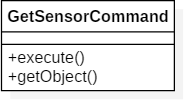
\includegraphics[width=0.2\linewidth]{images/core/classes/GetSensorCommand}
\end{figure}
\subsubsection{Declaration}{
\begin{lstlisting}[frame=none]
public class GetSensorCommand
 extends java.lang.Object implements RequestCommand\end{lstlisting}
\subsubsection{Constructor summary}{
\begin{verse}
\hyperlink{CommandRequestPattern.GetSensorCommand()}{{\bf GetSensorCommand()}} Default constructor\\
\end{verse}
}
\subsubsection{Method summary}{
\begin{verse}
\hyperlink{CommandRequestPattern.GetSensorCommand.execute()}{{\bf execute()}} This is the Execution form the requested Command.\\
\hyperlink{CommandRequestPattern.GetSensorCommand.getObject()}{{\bf getObject()}} This Method Return the Requested Sensor as a KStream\\
\end{verse}
}
\subsubsection{Constructors}{
\vskip -2em
\begin{itemize}
\item{ 
\index{GetSensorCommand()}
\hypertarget{CommandRequestPattern.GetSensorCommand()}{{\bf  GetSensorCommand}\\}
\begin{lstlisting}[frame=none]
public GetSensorCommand()\end{lstlisting} %end signature
\begin{itemize}
\item{
{\bf  Description}

Default constructor
}
\end{itemize}
}%end item
\end{itemize}
}
\subsubsection{Methods}{
\vskip -2em
\begin{itemize}
\item{ 
\index{execute()}
\hypertarget{CommandRequestPattern.GetSensorCommand.execute()}{{\bf  execute}\\}
\begin{lstlisting}[frame=none]
public void execute()\end{lstlisting} %end signature
\begin{itemize}
\item{
{\bf  Description}

This is the Execution form the requested Command. So it will search for the Sensor Uid
}
\end{itemize}
}%end item
\item{ 
\index{getObject()}
\hypertarget{CommandRequestPattern.GetSensorCommand.getObject()}{{\bf  getObject}\\}
\begin{lstlisting}[frame=none]
public void getObject()\end{lstlisting} %end signature
\begin{itemize}
\item{
{\bf  Description}

This Method Return the Requested Sensor as a KStream
}
\end{itemize}
}%end item
\end{itemize}
}
}
\subsection{\label{CommandRequestPattern.GetTileCommand}Class GetTileCommand}{
\hypertarget{CommandRequestPattern.GetTileCommand}{}\vskip .1in 
This Command request a Tile in the System.\vskip .1in 
\begin{figure}[!hbp]
	\centering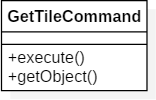
\includegraphics[width=0.2\linewidth]{images/core/classes/GetTileCommand}
\end{figure} 
\subsubsection{Declaration}{
\begin{lstlisting}[frame=none]
public class GetTileCommand
 extends java.lang.Object implements RequestCommand\end{lstlisting}
\subsubsection{Constructor summary}{
\begin{verse}
\hyperlink{CommandRequestPattern.GetTileCommand()}{{\bf GetTileCommand()}} Default constructor\\
\end{verse}
}
\subsubsection{Method summary}{
\begin{verse}
\hyperlink{CommandRequestPattern.GetTileCommand.execute()}{{\bf execute()}} This is the Execution form the requested Command.\\
\hyperlink{CommandRequestPattern.GetTileCommand.getObject()}{{\bf getObject()}} This Method Return the Requested Tile as a KStream\\
\end{verse}
}
\subsubsection{Constructors}{
\vskip -2em
\begin{itemize}
\item{ 
\index{GetTileCommand()}
\hypertarget{CommandRequestPattern.GetTileCommand()}{{\bf  GetTileCommand}\\}
\begin{lstlisting}[frame=none]
public GetTileCommand()\end{lstlisting} %end signature
\begin{itemize}
\item{
{\bf  Description}

Default constructor
}
\end{itemize}
}%end item
\end{itemize}
}
\subsubsection{Methods}{
\vskip -2em
\begin{itemize}
\item{ 
\index{execute()}
\hypertarget{CommandRequestPattern.GetTileCommand.execute()}{{\bf  execute}\\}
\begin{lstlisting}[frame=none]
public void execute()\end{lstlisting} %end signature
\begin{itemize}
\item{
{\bf  Description}

This is the Execution form the requested Command. So it will search for the Tile
}
\end{itemize}
}%end item
\item{ 
\index{getObject()}
\hypertarget{CommandRequestPattern.GetTileCommand.getObject()}{{\bf  getObject}\\}
\begin{lstlisting}[frame=none]
public void getObject()\end{lstlisting} %end signature
\begin{itemize}
\item{
{\bf  Description}

This Method Return the Requested Tile as a KStream
}
\end{itemize}
}%end item
\end{itemize}
}
}
\subsection{\label{CommandRequestPattern.Replier}Class Replier}{
\hypertarget{CommandRequestPattern.Replier}{}\vskip .1in 
This Class handels the Requests and Replies to them\vskip .1in
\begin{figure}[!hbp]
	\centering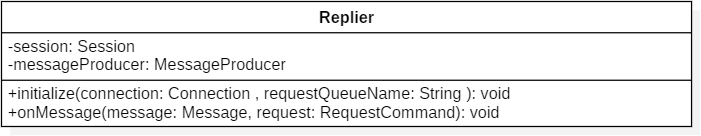
\includegraphics[width=0.8\linewidth]{images/core/classes/Replier}
\end{figure}
\subsubsection{Declaration}{
\begin{lstlisting}[frame=none]
public class Replier
 extends java.lang.Object\end{lstlisting}
\subsubsection{Constructor summary}{
\begin{verse}
\hyperlink{CommandRequestPattern.Replier()}{{\bf Replier()}} Default constructor\\
\end{verse}
}
\subsubsection{Method summary}{
\begin{verse}
\hyperlink{CommandRequestPattern.Replier.initialize(Connection, java.lang.String)}{{\bf initialize(Connection, String)}} This is the initialisation Method for the Replier to connect to different Requestors\\
\hyperlink{CommandRequestPattern.Replier.onMessage(Message, CommandRequestPattern.RequestCommand)}{{\bf onMessage(Message, RequestCommand)}} This Methode triggers something in the System waht has to be done\\
\end{verse}
}
\subsubsection{Constructors}{
\vskip -2em
\begin{itemize}
\item{ 
\index{Replier()}
\hypertarget{CommandRequestPattern.Replier()}{{\bf  Replier}\\}
\begin{lstlisting}[frame=none]
public Replier()\end{lstlisting} %end signature
\begin{itemize}
\item{
{\bf  Description}

Default constructor
}
\end{itemize}
}%end item
\end{itemize}
}
\subsubsection{Methods}{
\vskip -2em
\begin{itemize}
\item{ 
\index{initialize(Connection, String)}
\hypertarget{CommandRequestPattern.Replier.initialize(Connection, java.lang.String)}{{\bf  initialize}\\}
\begin{lstlisting}[frame=none]
public void initialize(Connection connection,java.lang.String requestQueueName)\end{lstlisting} %end signature
\begin{itemize}
\item{
{\bf  Description}

This is the initialisation Method for the Replier to connect to different Requestors
}
\item{
{\bf  Parameters}
  \begin{itemize}
   \item{
\texttt{connection} -- This is the Connection parameter, so taht the replier knows where he answers}
   \item{
\texttt{requestQueueName} -- This a Simple name for the request Queue}
  \end{itemize}
}%end item
\end{itemize}
}%end item
\item{ 
\index{onMessage(Message, RequestCommand)}
\hypertarget{CommandRequestPattern.Replier.onMessage(Message, CommandRequestPattern.RequestCommand)}{{\bf  onMessage}\\}
\begin{lstlisting}[frame=none]
public void onMessage(Message message,RequestCommand request)\end{lstlisting} %end signature
\begin{itemize}
\item{
{\bf  Description}

This Methode triggers something in the System waht has to be done
}
\item{
{\bf  Parameters}
  \begin{itemize}
   \item{
\texttt{message} -- This is a simple Message parameter}
   \item{
\texttt{request} -- This is the RequestCommand Object wich Contains the Real request.}
  \end{itemize}
}%end item
\end{itemize}
}%end item
\end{itemize}
}
}
\subsection{\label{CommandRequestPattern.Requestor}Class Requestor}{
\hypertarget{CommandRequestPattern.Requestor}{}\vskip .1in 
The Implemente this class and request something to the System and a Replier answer to it.\vskip .1in 
\begin{figure}[!hbp]
	\centering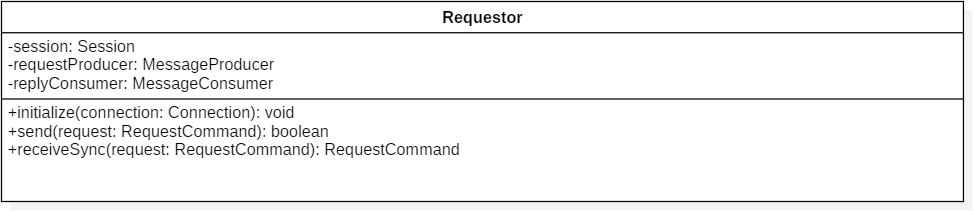
\includegraphics[width=0.8\linewidth]{images/core/classes/Requestor}
\end{figure}
\subsubsection{Declaration}{
\begin{lstlisting}[frame=none]
public class Requestor
 extends java.lang.Object\end{lstlisting}
\subsubsection{Constructor summary}{
\begin{verse}
\hyperlink{CommandRequestPattern.Requestor()}{{\bf Requestor()}} Default constructor\\
\end{verse}
}
\subsubsection{Method summary}{
\begin{verse}
\hyperlink{CommandRequestPattern.Requestor.initialize(Connection)}{{\bf initialize(Connection)}} \\
\hyperlink{CommandRequestPattern.Requestor.receiveSync(CommandRequestPattern.RequestCommand)}{{\bf receiveSync(RequestCommand)}} This Methode is there to got the Request again when it get lost or something\\
\hyperlink{CommandRequestPattern.Requestor.send(CommandRequestPattern.RequestCommand)}{{\bf send(RequestCommand)}} \\
\end{verse}
}
\subsubsection{Constructors}{
\vskip -2em
\begin{itemize}
\item{ 
\index{Requestor()}
\hypertarget{CommandRequestPattern.Requestor()}{{\bf  Requestor}\\}
\begin{lstlisting}[frame=none]
public Requestor()\end{lstlisting} %end signature
\begin{itemize}
\item{
{\bf  Description}

Default constructor
}
\end{itemize}
}%end item
\end{itemize}
}
\subsubsection{Methods}{
\vskip -2em
\begin{itemize}
\item{ 
\index{initialize(Connection)}
\hypertarget{CommandRequestPattern.Requestor.initialize(Connection)}{{\bf  initialize}\\}
\begin{lstlisting}[frame=none]
public void initialize(Connection connection)\end{lstlisting} %end signature
\begin{itemize}
\item{
{\bf  Parameters}
  \begin{itemize}
   \item{
\texttt{connection} -- This is the Connection parameter, so taht the repuestor knows where he requests something}
  \end{itemize}
}%end item
\end{itemize}
}%end item
\item{ 
\index{receiveSync(RequestCommand)}
\hypertarget{CommandRequestPattern.Requestor.receiveSync(CommandRequestPattern.RequestCommand)}{{\bf  receiveSync}\\}
\begin{lstlisting}[frame=none]
public RequestCommand receiveSync(RequestCommand request)\end{lstlisting} %end signature
\begin{itemize}
\item{
{\bf  Description}

This Methode is there to got the Request again when it get lost or something
}
\item{
{\bf  Parameters}
  \begin{itemize}
   \item{
\texttt{request} -- It Returns the Requested RequestCommand}
  \end{itemize}
}%end item
\item{{\bf  Returns} -- 
A RequestCommand which contains a Request for a RequestCommand 
}%end item
\end{itemize}
}%end item
\item{ 
\index{send(RequestCommand)}
\hypertarget{CommandRequestPattern.Requestor.send(CommandRequestPattern.RequestCommand)}{{\bf  send}\\}
\begin{lstlisting}[frame=none]
public boolean send(RequestCommand request)\end{lstlisting} %end signature
\begin{itemize}
\item{
{\bf  Parameters}
  \begin{itemize}
   \item{
\texttt{request} -- This is the RequestCommand Object wich Conntains the Real request.}
  \end{itemize}
}%end item
\item{{\bf  Returns} -- 
true if the RequestCommand got send and false otherwise 
}%end item
\end{itemize}
}%end item
\end{itemize}
}
}
}
\section{Package ConfigGUI}{
\label{ConfigGUI}\hypertarget{ConfigGUI}{}
\hskip -.05in
\hbox to \hsize{\textit{ Package Contents\hfil Page}}
\vskip .13in
\hbox{{\bf  Classes}}
\entityintro{DeleteFrame}{ConfigGUI.DeleteFrame}{This Frame is the Delete Frame, where you delete Topics out of the Programm}
\entityintro{JFrame}{ConfigGUI.JFrame}{This is the Basic Interface from Java for building a Frame.}
\entityintro{MainFrame}{ConfigGUI.MainFrame}{This Class holds the main functionality of the PaVoS program.}
\entityintro{SensorFrame}{ConfigGUI.SensorFrame}{This Frame hold the data of all possible Sensors in the System.}
\vskip .1in
\vskip .1in
\subsection{\label{ConfigGUI.DeleteFrame}Class DeleteFrame}{
\hypertarget{ConfigGUI.DeleteFrame}{}\vskip .1in 
This Frame is the Delete Frame, where you delete Topics out of the Programm\vskip .1in 
\begin{figure}[!hbp]
	\centering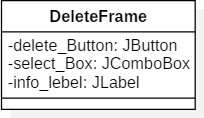
\includegraphics[width=0.2\linewidth]{images/core/classes/DeleteFrame}
\end{figure}
\subsubsection{Declaration}{
\begin{lstlisting}[frame=none]
public class DeleteFrame
 extends ConfigGUI.JFrame\end{lstlisting}
\subsubsection{Constructor summary}{
\begin{verse}
\hyperlink{ConfigGUI.DeleteFrame()}{{\bf DeleteFrame()}} Default constructor\\
\end{verse}
}
\subsubsection{Constructors}{
\vskip -2em
\begin{itemize}
\item{ 
\index{DeleteFrame()}
\hypertarget{ConfigGUI.DeleteFrame()}{{\bf  DeleteFrame}\\}
\begin{lstlisting}[frame=none]
public DeleteFrame()\end{lstlisting} %end signature
\begin{itemize}
\item{
{\bf  Description}

Default constructor
}
\end{itemize}
}%end item
\end{itemize}
}
}
\subsection{\label{ConfigGUI.JFrame}Class JFrame}{
\hypertarget{ConfigGUI.JFrame}{}\vskip .1in 
This is the Basic Interface from Java for building a Frame.\vskip .1in 
\begin{figure}[!hbp]
	\centering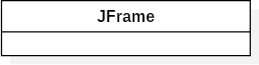
\includegraphics[width=0.2\linewidth]{images/core/classes/JFrame}
\end{figure}
\subsubsection{Declaration}{
\begin{lstlisting}[frame=none]
public class JFrame
 extends java.lang.Object\end{lstlisting}
\subsubsection{All known subclasses}{SensorFrame\small{\refdefined{ConfigGUI.SensorFrame}}, MainFrame\small{\refdefined{ConfigGUI.MainFrame}}, DeleteFrame\small{\refdefined{ConfigGUI.DeleteFrame}}}
\subsubsection{Constructor summary}{
\begin{verse}
\hyperlink{ConfigGUI.JFrame()}{{\bf JFrame()}} Default constructor\\
\end{verse}
}
\subsubsection{Constructors}{
\vskip -2em
\begin{itemize}
\item{ 
\index{JFrame()}
\hypertarget{ConfigGUI.JFrame()}{{\bf  JFrame}\\}
\begin{lstlisting}[frame=none]
public JFrame()\end{lstlisting} %end signature
\begin{itemize}
\item{
{\bf  Description}

Default constructor
}
\end{itemize}
}%end item
\end{itemize}
}
}
\subsection{\label{ConfigGUI.MainFrame}Class MainFrame}{
\hypertarget{ConfigGUI.MainFrame}{}\vskip .1in 
This Class holds the main functionality of the PaVoS program. It starts/stops the whole System and manages the export/import.\vskip .1in 
\begin{figure}[!hbp]
	\centering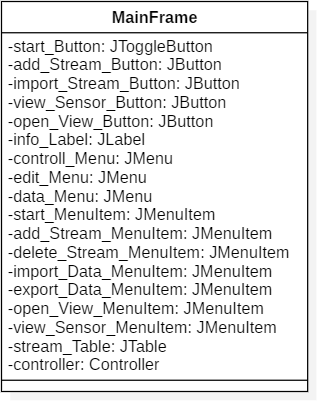
\includegraphics[width=0.4\linewidth]{images/core/classes/MainFrame}
\end{figure}
\subsubsection{Declaration}{
\begin{lstlisting}[frame=none]
public class MainFrame
 extends ConfigGUI.JFrame\end{lstlisting}
\subsubsection{Constructor summary}{
\begin{verse}
\hyperlink{ConfigGUI.MainFrame()}{{\bf MainFrame()}} Default constructor\\
\end{verse}
}
\subsubsection{Constructors}{
\vskip -2em
\begin{itemize}
\item{ 
\index{MainFrame()}
\hypertarget{ConfigGUI.MainFrame()}{{\bf  MainFrame}\\}
\begin{lstlisting}[frame=none]
public MainFrame()\end{lstlisting} %end signature
\begin{itemize}
\item{
{\bf  Description}

Default constructor
}
\end{itemize}
}%end item
\end{itemize}
}
}
\subsection{\label{ConfigGUI.SensorFrame}Class SensorFrame}{
\hypertarget{ConfigGUI.SensorFrame}{}\vskip .1in 
This Frame hold the data of all possible Sensors in the System.\vskip .1in 

\begin{figure}[!hbp]
	\centering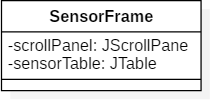
\includegraphics[width=0.2\linewidth]{images/core/classes/SensorFrame}
\end{figure}


\subsubsection{Declaration}{
\begin{lstlisting}[frame=none]
public class SensorFrame
 extends ConfigGUI.JFrame\end{lstlisting}
\subsubsection{Constructor summary}{
\begin{verse}
\hyperlink{ConfigGUI.SensorFrame()}{{\bf SensorFrame()}} Default constructor\\
\end{verse}
}
\subsubsection{Constructors}{
\vskip -2em
\begin{itemize}
\item{ 
\index{SensorFrame()}
\hypertarget{ConfigGUI.SensorFrame()}{{\bf  SensorFrame}\\}
\begin{lstlisting}[frame=none]
public SensorFrame()\end{lstlisting} %end signature
\begin{itemize}
\item{
{\bf  Description}

Default constructor
}
\end{itemize}
}%end item
\end{itemize}
}
}
}
\section{Package Controller}{
\label{Controller}\hypertarget{Controller}{}
\hskip -.05in
\hbox to \hsize{\textit{ Package Contents\hfil Page}}
\vskip .13in
\hbox{{\bf  Classes}}
\entityintro{ClusterProcessStrategy}{Controller.ClusterProcessStrategy}{This Class is for the generation of the Clusters for the View.}
\entityintro{CombinerProcessStrategy}{Controller.CombinerProcessStrategy}{This Class does combinate the Clusters to bigger Cluster for the Different Zoom Levels}
\entityintro{Controller}{Controller.Controller}{This Class is the ControllerClass which manages the Requests and start new TopologyBuilders to start new Processing Application.}
\entityintro{ExportProcessStrategy}{Controller.ExportProcessStrategy}{This Class is for The Processing of the Export Stream and it generates a Output Stream}
\entityintro{GraphiteProcessStrategy}{Controller.GraphiteProcessStrategy}{This Class is for The Processing of the Data for Graphite, to represente the Sensors.}
\entityintro{TopologyBuilder}{Controller.TopologyBuilder}{A component that is used to build a ProcessorTopology.}
\entityintro{UncaughtExceptionHandler}{Controller.UncaughtExceptionHandler}{To catch any unexpected exceptions, you can set before you start the application.}
\vskip .1in
\vskip .1in
\subsection{\label{Controller.ClusterProcessStrategy}Class ClusterProcessStrategy}{
\hypertarget{Controller.ClusterProcessStrategy}{}\vskip .1in 
This Class is for the generation of the Clusters for the View. It Generates a Cluster Outputtopic\vskip .1in 
\begin{figure}[!hbp]
	\centering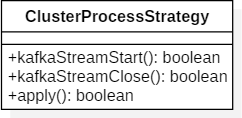
\includegraphics[width=0.4\linewidth]{images/core/classes/ClusterProcessStrategy}
\end{figure}
\subsubsection{Declaration}{
\begin{lstlisting}[frame=none]
public class ClusterProcessStrategy
 extends java.lang.Object\end{lstlisting}
\subsubsection{Constructor summary}{
\begin{verse}
\hyperlink{Controller.ClusterProcessStrategy()}{{\bf ClusterProcessStrategy()}} Default constructor\\
\end{verse}
}
\subsubsection{Method summary}{
\begin{verse}
\hyperlink{Controller.ClusterProcessStrategy.apply()}{{\bf apply()}} This Methode definite the Process of the Application.\\
\hyperlink{Controller.ClusterProcessStrategy.kafkaStreamClose()}{{\bf kafkaStreamClose()}} This Method is used to explicitly close the Kafka Stream thread.\\
\hyperlink{Controller.ClusterProcessStrategy.kafkaStreamStart()}{{\bf kafkaStreamStart()}} This Method is used to explicitly start the Kafka Stream thread.\\
\end{verse}
}
\subsubsection{Constructors}{
\vskip -2em
\begin{itemize}
\item{ 
\index{ClusterProcessStrategy()}
\hypertarget{Controller.ClusterProcessStrategy()}{{\bf  ClusterProcessStrategy}\\}
\begin{lstlisting}[frame=none]
public ClusterProcessStrategy()\end{lstlisting} %end signature
\begin{itemize}
\item{
{\bf  Description}

Default constructor
}
\end{itemize}
}%end item
\end{itemize}
}
\subsubsection{Methods}{
\vskip -2em
\begin{itemize}
\item{ 
\index{apply()}
\hypertarget{Controller.ClusterProcessStrategy.apply()}{{\bf  apply}\\}
\begin{lstlisting}[frame=none]
public boolean apply()\end{lstlisting} %end signature
\begin{itemize}
\item{
{\bf  Description}

This Methode definite the Process of the Application. What Application does specificly.
}
\item{{\bf  Returns} -- 
true if the Cluster Process got Successfully worked, false otherwise 
}%end item
\end{itemize}
}%end item
\item{ 
\index{kafkaStreamClose()}
\hypertarget{Controller.ClusterProcessStrategy.kafkaStreamClose()}{{\bf  kafkaStreamClose}\\}
\begin{lstlisting}[frame=none]
public boolean kafkaStreamClose()\end{lstlisting} %end signature
\begin{itemize}
\item{
{\bf  Description}

This Method is used to explicitly close the Kafka Stream thread. So that the Processing stops.
}
\item{{\bf  Returns} -- 
true if the Kafka Stream closed false otherwise 
}%end item
\end{itemize}
}%end item
\item{ 
\index{kafkaStreamStart()}
\hypertarget{Controller.ClusterProcessStrategy.kafkaStreamStart()}{{\bf  kafkaStreamStart}\\}
\begin{lstlisting}[frame=none]
public boolean kafkaStreamStart()\end{lstlisting} %end signature
\begin{itemize}
\item{
{\bf  Description}

This Method is used to explicitly start the Kafka Stream thread. So that theProcessing need to get started.
}
\item{{\bf  Returns} -- 
true if the Kafka Stream Started, false otherwise 
}%end item
\end{itemize}
}%end item
\end{itemize}
}
}
\subsection{\label{Controller.CombinerProcessStrategy}Class CombinerProcessStrategy}{
\hypertarget{Controller.CombinerProcessStrategy}{}\vskip .1in 
This Class does combinate the Clusters to bigger Cluster for the Different Zoom Levels\vskip .1in 
\begin{figure}[!hbp]
	\centering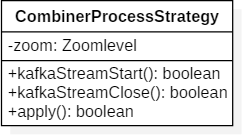
\includegraphics[width=0.2\linewidth]{images/core/classes/CombinerProcessStrategy}
\end{figure}
\subsubsection{Declaration}{
\begin{lstlisting}[frame=none]
public class CombinerProcessStrategy
 extends java.lang.Object\end{lstlisting}
\subsubsection{Constructor summary}{
\begin{verse}
\hyperlink{Controller.CombinerProcessStrategy()}{{\bf CombinerProcessStrategy()}} Default constructor\\
\end{verse}
}
\subsubsection{Method summary}{
\begin{verse}
\hyperlink{Controller.CombinerProcessStrategy.apply()}{{\bf apply()}} This Methode definite the Process of the Application.\\
\hyperlink{Controller.CombinerProcessStrategy.kafkaStreamClose()}{{\bf kafkaStreamClose()}} This Method is used to explicitly close the Kafka Stream thread.\\
\hyperlink{Controller.CombinerProcessStrategy.kafkaStreamStart()}{{\bf kafkaStreamStart()}} This Method is used to explicitly start the Kafka Stream thread.\\
\end{verse}
}
\subsubsection{Constructors}{
\vskip -2em
\begin{itemize}
\item{ 
\index{CombinerProcessStrategy()}
\hypertarget{Controller.CombinerProcessStrategy()}{{\bf  CombinerProcessStrategy}\\}
\begin{lstlisting}[frame=none]
public CombinerProcessStrategy()\end{lstlisting} %end signature
\begin{itemize}
\item{
{\bf  Description}

Default constructor
}
\end{itemize}
}%end item
\end{itemize}
}
\subsubsection{Methods}{
\vskip -2em
\begin{itemize}
\item{ 
\index{apply()}
\hypertarget{Controller.CombinerProcessStrategy.apply()}{{\bf  apply}\\}
\begin{lstlisting}[frame=none]
public boolean apply()\end{lstlisting} %end signature
\begin{itemize}
\item{
{\bf  Description}

This Methode definite the Process of the Application. What Application does specificly.
}
\item{{\bf  Returns} -- 
true if the Combiner Process got Successfully worked 
}%end item
\end{itemize}
}%end item
\item{ 
\index{kafkaStreamClose()}
\hypertarget{Controller.CombinerProcessStrategy.kafkaStreamClose()}{{\bf  kafkaStreamClose}\\}
\begin{lstlisting}[frame=none]
public boolean kafkaStreamClose()\end{lstlisting} %end signature
\begin{itemize}
\item{
{\bf  Description}

This Method is used to explicitly close the Kafka Stream thread. So that the Processing stops.
}
\item{{\bf  Returns} -- 
true if the Kafka Stream closed, false otherwise 
}%end item
\end{itemize}
}%end item
\item{ 
\index{kafkaStreamStart()}
\hypertarget{Controller.CombinerProcessStrategy.kafkaStreamStart()}{{\bf  kafkaStreamStart}\\}
\begin{lstlisting}[frame=none]
public boolean kafkaStreamStart()\end{lstlisting} %end signature
\begin{itemize}
\item{
{\bf  Description}

This Method is used to explicitly start the Kafka Stream thread. So that theProcessing need to get started.
}
\item{{\bf  Returns} -- 
true if the Kafka Stream Started false otherwise 
}%end item
\end{itemize}
}%end item
\end{itemize}
}
}
\subsection{\label{Controller.Controller}Class Controller}{
\hypertarget{Controller.Controller}{}\vskip .1in 
This Class is the ControllerClass which manages the Requests and start new TopologyBuilders to start new Processing Application.\vskip .1in 
\begin{figure}[!hbp]
	\centering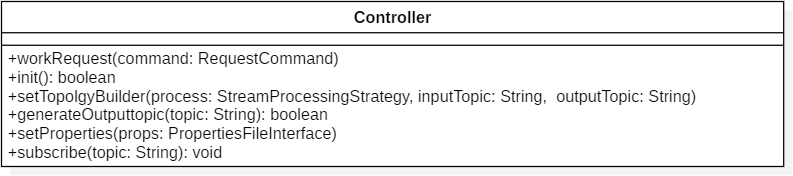
\includegraphics[width=0.5\linewidth]{images/core/classes/Controller}
\end{figure}
\subsubsection{Declaration}{
\begin{lstlisting}[frame=none]
public class Controller
 extends java.lang.Object\end{lstlisting}
\subsubsection{Constructor summary}{
\begin{verse}
\hyperlink{Controller.Controller()}{{\bf Controller()}} Default constructor\\
\end{verse}
}
\subsubsection{Method summary}{
\begin{verse}
\hyperlink{Controller.Controller.generateOutputtopic(java.lang.String)}{{\bf generateOutputtopic(String)}} This Method generates a Output Topic, which uses a ProcessApplikation as OutputSink.\\
\hyperlink{Controller.Controller.init()}{{\bf init()}} This Method initialise the Controler\\
\hyperlink{Controller.Controller.setProperties(PropertiesFileInterface)}{{\bf setProperties(PropertiesFileInterface)}} This Method sets the Properties File\\
\hyperlink{Controller.Controller.setTopolgyBuilder(StreamProcessingStrategy, java.lang.String, java.lang.String)}{{\bf setTopolgyBuilder(StreamProcessingStrategy, String, String)}} Thsi Method starts a TopolgyBuilder to start a Kafka Stream Process.\\
\hyperlink{Controller.Controller.subscribe(java.lang.String)}{{\bf subscribe(String)}} This method subscribe the controller to the Input Kafka Stream\\
\hyperlink{Controller.Controller.workRequest(RequestCommand)}{{\bf workRequest(RequestCommand)}} This Method process the single Reuqest form the View\\
\end{verse}
}
\subsubsection{Constructors}{
\vskip -2em
\begin{itemize}
\item{ 
\index{Controller()}
\hypertarget{Controller.Controller()}{{\bf  Controller}\\}
\begin{lstlisting}[frame=none]
public Controller()\end{lstlisting} %end signature
\begin{itemize}
\item{
{\bf  Description}

Default constructor
}
\end{itemize}
}%end item
\end{itemize}
}
\subsubsection{Methods}{
\vskip -2em
\begin{itemize}
\item{ 
\index{generateOutputtopic(String)}
\hypertarget{Controller.Controller.generateOutputtopic(java.lang.String)}{{\bf  generateOutputtopic}\\}
\begin{lstlisting}[frame=none]
public boolean generateOutputtopic(java.lang.String topic)\end{lstlisting} %end signature
\begin{itemize}
\item{
{\bf  Description}

This Method generates a Output Topic, which uses a ProcessApplikation as OutputSink. This will use Apache Avro Format.
}
\item{
{\bf  Parameters}
  \begin{itemize}
   \item{
\texttt{topic} -- topic name of the new Topic in Kafka}
  \end{itemize}
}%end item
\item{{\bf  Returns} -- 
true when the Output Topic got successful generated 
}%end item
\end{itemize}
}%end item
\item{ 
\index{init()}
\hypertarget{Controller.Controller.init()}{{\bf  init}\\}
\begin{lstlisting}[frame=none]
public boolean init()\end{lstlisting} %end signature
\begin{itemize}
\item{
{\bf  Description}

This Method initialise the Controler
}
\item{{\bf  Returns} -- 
true when the initialise was successful and false otherwise 
}%end item
\end{itemize}
}%end item
\item{ 
\index{setProperties(PropertiesFileInterface)}
\hypertarget{Controller.Controller.setProperties(PropertiesFileInterface)}{{\bf  setProperties}\\}
\begin{lstlisting}[frame=none]
public void setProperties(PropertiesFileInterface props)\end{lstlisting} %end signature
\begin{itemize}
\item{
{\bf  Description}

This Method sets the Properties File
}
\item{
{\bf  Parameters}
  \begin{itemize}
   \item{
\texttt{props} -- props is the Propertyfile form where the controller reads his Settings}
  \end{itemize}
}%end item
\end{itemize}
}%end item
\item{ 
\index{setTopolgyBuilder(StreamProcessingStrategy, String, String)}
\hypertarget{Controller.Controller.setTopolgyBuilder(StreamProcessingStrategy, java.lang.String, java.lang.String)}{{\bf  setTopolgyBuilder}\\}
\begin{lstlisting}[frame=none]
public void setTopolgyBuilder(StreamProcessingStrategy process,java.lang.String inputTopic,java.lang.String outputTopic)\end{lstlisting} %end signature
\begin{itemize}
\item{
{\bf  Description}

Thsi Method starts a TopolgyBuilder to start a Kafka Stream Process.
}
\item{
{\bf  Parameters}
  \begin{itemize}
   \item{
\texttt{process} -- process name of the Process Application}
   \item{
\texttt{inputTopic} -- inputTopic of the Kafka Topic}
   \item{
\texttt{outputTopic} -- outputTopic of the Kafka Topic}
  \end{itemize}
}%end item
\end{itemize}
}%end item
\item{ 
\index{subscribe(String)}
\hypertarget{Controller.Controller.subscribe(java.lang.String)}{{\bf  subscribe}\\}
\begin{lstlisting}[frame=none]
public void subscribe(java.lang.String topic)\end{lstlisting} %end signature
\begin{itemize}
\item{
{\bf  Description}

This method subscribe the controller to the Input Kafka Stream
}
\item{
{\bf  Parameters}
  \begin{itemize}
   \item{
\texttt{topic} -- The Name of the Topic which you want to subscribe}
  \end{itemize}
}%end item
\end{itemize}
}%end item
\item{ 
\index{workRequest(RequestCommand)}
\hypertarget{Controller.Controller.workRequest(RequestCommand)}{{\bf  workRequest}\\}
\begin{lstlisting}[frame=none]
public void workRequest(RequestCommand command)\end{lstlisting} %end signature
\begin{itemize}
\item{
{\bf  Description}

This Method process the single Reuqest form the View
}
\item{
{\bf  Parameters}
  \begin{itemize}
   \item{
\texttt{command} -- command is Instance of the RequestCommand Interface which contains a Job Request}
  \end{itemize}
}%end item
\end{itemize}
}%end item
\end{itemize}
}
}
\subsection{\label{Controller.ExportProcessStrategy}Class ExportProcessStrategy}{
\hypertarget{Controller.ExportProcessStrategy}{}\vskip .1in 
This Class is for The Processing of the Export Stream and it generates a Output Stream\vskip .1in
\begin{figure}[!hbp]
	\centering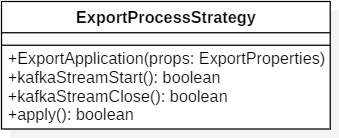
\includegraphics[width=0.4\linewidth]{images/core/classes/ExportProcessStrategy}
\end{figure} 
\subsubsection{Declaration}{
\begin{lstlisting}[frame=none]
public class ExportProcessStrategy
 extends java.lang.Object\end{lstlisting}
\subsubsection{Constructor summary}{
\begin{verse}
\hyperlink{Controller.ExportProcessStrategy()}{{\bf ExportProcessStrategy()}} Default constructor\\
\end{verse}
}
\subsubsection{Method summary}{
\begin{verse}
\hyperlink{Controller.ExportProcessStrategy.apply()}{{\bf apply()}} This Methode definite the Process of the Application.\\
\hyperlink{Controller.ExportProcessStrategy.ExportApplication(ExportProperties)}{{\bf ExportApplication(ExportProperties)}} This is the default Contructer for the Export Process\\
\hyperlink{Controller.ExportProcessStrategy.kafkaStreamClose()}{{\bf kafkaStreamClose()}} This Method is used to explicitly close the Kafka Stream thread.\\
\hyperlink{Controller.ExportProcessStrategy.kafkaStreamStart()}{{\bf kafkaStreamStart()}} This Method is used to explicitly start the Kafka Stream thread.\\
\end{verse}
}
\subsubsection{Constructors}{
\vskip -2em
\begin{itemize}
\item{ 
\index{ExportProcessStrategy()}
\hypertarget{Controller.ExportProcessStrategy()}{{\bf  ExportProcessStrategy}\\}
\begin{lstlisting}[frame=none]
public ExportProcessStrategy()\end{lstlisting} %end signature
\begin{itemize}
\item{
{\bf  Description}

Default constructor
}
\end{itemize}
}%end item
\end{itemize}
}
\subsubsection{Methods}{
\vskip -2em
\begin{itemize}
\item{ 
\index{apply()}
\hypertarget{Controller.ExportProcessStrategy.apply()}{{\bf  apply}\\}
\begin{lstlisting}[frame=none]
public boolean apply()\end{lstlisting} %end signature
\begin{itemize}
\item{
{\bf  Description}

This Methode definite the Process of the Application. What Application does specificly.
}
\item{{\bf  Returns} -- 
true if the Export Process got Successfully worked. 
}%end item
\end{itemize}
}%end item
\item{ 
\index{ExportApplication(ExportProperties)}
\hypertarget{Controller.ExportProcessStrategy.ExportApplication(ExportProperties)}{{\bf  ExportApplication}\\}
\begin{lstlisting}[frame=none]
public void ExportApplication(ExportProperties props)\end{lstlisting} %end signature
\begin{itemize}
\item{
{\bf  Description}

This is the default Contructer for the Export Process
}
\item{
{\bf  Parameters}
  \begin{itemize}
   \item{
\texttt{props} -- ExportProperties is the Properties Object for the Application}
  \end{itemize}
}%end item
\end{itemize}
}%end item
\item{ 
\index{kafkaStreamClose()}
\hypertarget{Controller.ExportProcessStrategy.kafkaStreamClose()}{{\bf  kafkaStreamClose}\\}
\begin{lstlisting}[frame=none]
public boolean kafkaStreamClose()\end{lstlisting} %end signature
\begin{itemize}
\item{
{\bf  Description}

This Method is used to explicitly close the Kafka Stream thread. So that the Processing stops.
}
\item{{\bf  Returns} -- 
true if the Kafka Stream Started false otherwise 
}%end item
\end{itemize}
}%end item
\item{ 
\index{kafkaStreamStart()}
\hypertarget{Controller.ExportProcessStrategy.kafkaStreamStart()}{{\bf  kafkaStreamStart}\\}
\begin{lstlisting}[frame=none]
public boolean kafkaStreamStart()\end{lstlisting} %end signature
\begin{itemize}
\item{
{\bf  Description}

This Method is used to explicitly start the Kafka Stream thread. So that theProcessing need to get started.
}
\item{{\bf  Returns} -- 
true if the Kafka Stream Started false otherwise 
}%end item
\end{itemize}
}%end item
\end{itemize}
}
}
\subsection{\label{Controller.GraphiteProcessStrategy}Class GraphiteProcessStrategy}{
\hypertarget{Controller.GraphiteProcessStrategy}{}\vskip .1in 
This Class is for The Processing of the Data for Graphite, to represente the Sensors. It Generates a Graphite Output Stream\vskip .1in 
\begin{figure}[!hbp]
	\centering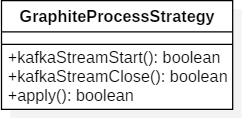
\includegraphics[width=0.2\linewidth]{images/core/classes/GraphiteProcessStrategy}
\end{figure} 
\subsubsection{Declaration}{
\begin{lstlisting}[frame=none]
public class GraphiteProcessStrategy
 extends java.lang.Object\end{lstlisting}
\subsubsection{Constructor summary}{
\begin{verse}
\hyperlink{Controller.GraphiteProcessStrategy()}{{\bf GraphiteProcessStrategy()}} Default constructor\\
\end{verse}
}
\subsubsection{Method summary}{
\begin{verse}
\hyperlink{Controller.GraphiteProcessStrategy.apply()}{{\bf apply()}} This Methode definite the Process of the Application.\\
\hyperlink{Controller.GraphiteProcessStrategy.kafkaStreamClose()}{{\bf kafkaStreamClose()}} This Method is used to explicitly close the Kafka Stream thread.\\
\hyperlink{Controller.GraphiteProcessStrategy.kafkaStreamStart()}{{\bf kafkaStreamStart()}} This Method is used to explicitly start the Kafka Stream thread.\\
\end{verse}
}
\subsubsection{Constructors}{
\vskip -2em
\begin{itemize}
\item{ 
\index{GraphiteProcessStrategy()}
\hypertarget{Controller.GraphiteProcessStrategy()}{{\bf  GraphiteProcessStrategy}\\}
\begin{lstlisting}[frame=none]
public GraphiteProcessStrategy()\end{lstlisting} %end signature
\begin{itemize}
\item{
{\bf  Description}

Default constructor
}
\end{itemize}
}%end item
\end{itemize}
}
\subsubsection{Methods}{
\vskip -2em
\begin{itemize}
\item{ 
\index{apply()}
\hypertarget{Controller.GraphiteProcessStrategy.apply()}{{\bf  apply}\\}
\begin{lstlisting}[frame=none]
public boolean apply()\end{lstlisting} %end signature
\begin{itemize}
\item{
{\bf  Description}

This Methode definite the Process of the Application. What Application does specificly.
}
\item{{\bf  Returns} -- 
true if the Graphite Process got Successfully worked 
}%end item
\end{itemize}
}%end item
\item{ 
\index{kafkaStreamClose()}
\hypertarget{Controller.GraphiteProcessStrategy.kafkaStreamClose()}{{\bf  kafkaStreamClose}\\}
\begin{lstlisting}[frame=none]
public boolean kafkaStreamClose()\end{lstlisting} %end signature
\begin{itemize}
\item{
{\bf  Description}

This Method is used to explicitly close the Kafka Stream thread. So that the Processing stops.
}
\item{{\bf  Returns} -- 
true if the Kafka Stream closed, false otherwise 
}%end item
\end{itemize}
}%end item
\item{ 
\index{kafkaStreamStart()}
\hypertarget{Controller.GraphiteProcessStrategy.kafkaStreamStart()}{{\bf  kafkaStreamStart}\\}
\begin{lstlisting}[frame=none]
public boolean kafkaStreamStart()\end{lstlisting} %end signature
\begin{itemize}
\item{
{\bf  Description}

This Method is used to explicitly start the Kafka Stream thread. So that theProcessing need to get started.
}
\item{{\bf  Returns} -- 
true if the Kafka Stream Started false otherwise 
}%end item
\end{itemize}
}%end item
\end{itemize}
}
}
\subsection{\label{Controller.TopologyBuilder}Class TopologyBuilder}{
\hypertarget{Controller.TopologyBuilder}{}\vskip .1in 
A component that is used to build a ProcessorTopology. A topology contains an acyclic graph of sources, processors, and sinks. A source is a node in the graph that consumes one or more Kafka topics and forwards them to its child nodes. A processor is a node in the graph that receives input records from upstream nodes, processes that records, and optionally forwarding new records to one or all of its children. Finally, a sink is a node in the graph that receives records from upstream nodes and writes them to a Kafka topic. This builder allows you to construct an acyclic graph of these nodes, and the builder is then passed into a new KafkaStreams instance that will then begin consuming, processing, and producing records\vskip .1in 
\begin{figure}[!hbp]
	\centering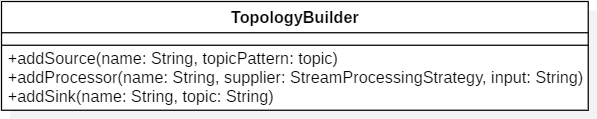
\includegraphics[width=0.4\linewidth]{images/core/classes/TopologyBuilder}
\end{figure}
\subsubsection{Declaration}{
\begin{lstlisting}[frame=none]
public class TopologyBuilder
 extends java.lang.Object\end{lstlisting}
\subsubsection{Constructor summary}{
\begin{verse}
\hyperlink{Controller.TopologyBuilder()}{{\bf TopologyBuilder()}} Default constructor\\
\end{verse}
}
\subsubsection{Method summary}{
\begin{verse}
\hyperlink{Controller.TopologyBuilder.addProcessor(java.lang.String, StreamProcessingStrategy, java.lang.String)}{{\bf addProcessor(String, StreamProcessingStrategy, String)}} Add a new processor node that receives and processes records output by one or more parent source or processor node.\\
\hyperlink{Controller.TopologyBuilder.addSink(java.lang.String, java.lang.String)}{{\bf addSink(String, String)}} Add a new sink that forwards records from upstream parent processor and/or source nodes to the named Kafka topic.\\
\hyperlink{Controller.TopologyBuilder.addSource(java.lang.String, topic)}{{\bf addSource(String, topic)}} Add a new source that consumes from topics matching the given pattern and forward the records to child processor and/or sink nodes.\\
\end{verse}
}
\subsubsection{Constructors}{
\vskip -2em
\begin{itemize}
\item{ 
\index{TopologyBuilder()}
\hypertarget{Controller.TopologyBuilder()}{{\bf  TopologyBuilder}\\}
\begin{lstlisting}[frame=none]
public TopologyBuilder()\end{lstlisting} %end signature
\begin{itemize}
\item{
{\bf  Description}

Default constructor
}
\end{itemize}
}%end item
\end{itemize}
}
\subsubsection{Methods}{
\vskip -2em
\begin{itemize}
\item{ 
\index{addProcessor(String, StreamProcessingStrategy, String)}
\hypertarget{Controller.TopologyBuilder.addProcessor(java.lang.String, StreamProcessingStrategy, java.lang.String)}{{\bf  addProcessor}\\}
\begin{lstlisting}[frame=none]
public void addProcessor(java.lang.String name,StreamProcessingStrategy supplier,java.lang.String input)\end{lstlisting} %end signature
\begin{itemize}
\item{
{\bf  Description}

Add a new processor node that receives and processes records output by one or more parent source or processor node.
}
\item{
{\bf  Parameters}
  \begin{itemize}
   \item{
\texttt{name} -- is the name of the Processor Stratgie}
   \item{
\texttt{supplier} -- supplier is the supplier of the Process instant to generate more then 1 Process}
   \item{
\texttt{input} -- input Topic Stream name}
  \end{itemize}
}%end item
\end{itemize}
}%end item
\item{ 
\index{addSink(String, String)}
\hypertarget{Controller.TopologyBuilder.addSink(java.lang.String, java.lang.String)}{{\bf  addSink}\\}
\begin{lstlisting}[frame=none]
public void addSink(java.lang.String name,java.lang.String topic)\end{lstlisting} %end signature
\begin{itemize}
\item{
{\bf  Description}

Add a new sink that forwards records from upstream parent processor and/or source nodes to the named Kafka topic.
}
\item{
{\bf  Parameters}
  \begin{itemize}
   \item{
\texttt{name} -- name of the Sink}
   \item{
\texttt{topic} -- name of the Topic Stream}
  \end{itemize}
}%end item
\end{itemize}
}%end item
\item{ 
\index{addSource(String, topic)}
\hypertarget{Controller.TopologyBuilder.addSource(java.lang.String, topic)}{{\bf  addSource}\\}
\begin{lstlisting}[frame=none]
public void addSource(java.lang.String name,topic topicPattern)\end{lstlisting} %end signature
\begin{itemize}
\item{
{\bf  Description}

Add a new source that consumes from topics matching the given pattern and forward the records to child processor and/or sink nodes.
}
\item{
{\bf  Parameters}
  \begin{itemize}
   \item{
\texttt{name} -- name of the Input Topic Stream}
   \item{
\texttt{topicPattern} -- topicPattern is a Pattern to filter the data from the Input Topic Stream}
  \end{itemize}
}%end item
\end{itemize}
}%end item
\end{itemize}
}
}
\subsection{\label{Controller.UncaughtExceptionHandler}Class UncaughtExceptionHandler}{
\hypertarget{Controller.UncaughtExceptionHandler}{}\vskip .1in 
To catch any unexpected exceptions, you can set before you start the application. This handler is called whenever a stream thread is terminated by an unexpected exception.\vskip .1in
\begin{figure}[!hbp]
	\centering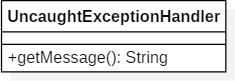
\includegraphics[width=0.2\linewidth]{images/core/classes/UncaughtExceptionHandler}
\end{figure} 
\subsubsection{Declaration}{
\begin{lstlisting}[frame=none]
public class UncaughtExceptionHandler
 extends java.lang.Object\end{lstlisting}
\subsubsection{Constructor summary}{
\begin{verse}
\hyperlink{Controller.UncaughtExceptionHandler()}{{\bf UncaughtExceptionHandler()}} Default constructor\\
\end{verse}
}
\subsubsection{Method summary}{
\begin{verse}
\hyperlink{Controller.UncaughtExceptionHandler.getMessage()}{{\bf getMessage()}} Returns the detail message string of this throwable.\\
\end{verse}
}
\subsubsection{Constructors}{
\vskip -2em
\begin{itemize}
\item{ 
\index{UncaughtExceptionHandler()}
\hypertarget{Controller.UncaughtExceptionHandler()}{{\bf  UncaughtExceptionHandler}\\}
\begin{lstlisting}[frame=none]
public UncaughtExceptionHandler()\end{lstlisting} %end signature
\begin{itemize}
\item{
{\bf  Description}

Default constructor
}
\end{itemize}
}%end item
\end{itemize}
}
\subsubsection{Methods}{
\vskip -2em
\begin{itemize}
\item{ 
\index{getMessage()}
\hypertarget{Controller.UncaughtExceptionHandler.getMessage()}{{\bf  getMessage}\\}
\begin{lstlisting}[frame=none]
public java.lang.String getMessage()\end{lstlisting} %end signature
\begin{itemize}
\item{
{\bf  Description}

Returns the detail message string of this throwable.
}
\item{{\bf  Returns} -- 
String with the error Message 
}%end item
\end{itemize}
}%end item
\end{itemize}
}
}
}
\section{Package Properties}{
\label{Properties}\hypertarget{Properties}{}
\hskip -.05in
\hbox to \hsize{\textit{ Package Contents\hfil Page}}
\vskip .13in
\hbox{{\bf  Interfaces}}
\entityintro{PropertiesFileInterface}{Properties.PropertiesFileInterface}{The Properties Interface is a special form of associative memory in which key-value pairs are always of type string.}
\vskip .13in
\hbox{{\bf  Classes}}
\entityintro{PropertiesFile}{Properties.PropertiesFile}{The Properties class is a special form of associative memory in which key-value pairs are always of type string.}
\vskip .1in
\vskip .1in
\subsection{\label{Properties.PropertiesFileInterface}Interface PropertiesFileInterface}{
\hypertarget{Properties.PropertiesFileInterface}{}\vskip .1in 
The Properties Interface is a special form of associative memory in which key-value pairs are always of type string. Since the entries can be stored in a file and read out again, hardwired character strings can be externalized from the program text so that the values ​​can be easily changed without retranslation.\vskip .1in 
\begin{figure}[!hbp]
	\centering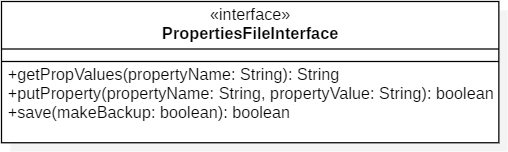
\includegraphics[width=0.4\linewidth]{images/core/classes/PropertiesFileInterface}
\end{figure} 
\subsubsection{Declaration}{
\begin{lstlisting}[frame=none]
public interface PropertiesFileInterface
\end{lstlisting}
\subsubsection{All known subinterfaces}{PropertiesFile\small{\refdefined{Properties.PropertiesFile}}}
\subsubsection{All classes known to implement interface}{PropertiesFile\small{\refdefined{Properties.PropertiesFile}}}
\subsubsection{Method summary}{
\begin{verse}
\hyperlink{Properties.PropertiesFileInterface.getPropValues(java.lang.String)}{{\bf getPropValues(String)}} This Methodes returns the requestet propertie Value\\
\hyperlink{Properties.PropertiesFileInterface.putProperty(java.lang.String, java.lang.String)}{{\bf putProperty(String, String)}} The Method adds a key-value pair to the Properties object.\\
\hyperlink{Properties.PropertiesFileInterface.save(boolean)}{{\bf save(boolean)}} This Method saves the PropertiesFile with the Option to do a Backup of the File\\
\end{verse}
}
\subsubsection{Methods}{
\vskip -2em
\begin{itemize}
\item{ 
\index{getPropValues(String)}
\hypertarget{Properties.PropertiesFileInterface.getPropValues(java.lang.String)}{{\bf  getPropValues}\\}
\begin{lstlisting}[frame=none]
java.lang.String getPropValues(java.lang.String propertyName)\end{lstlisting} %end signature
\begin{itemize}
\item{
{\bf  Description}

This Methodes returns the requestet propertie Value
}
\item{
{\bf  Parameters}
  \begin{itemize}
   \item{
\texttt{propertyName} -- propertyName is the name of the Requested Property}
  \end{itemize}
}%end item
\item{{\bf  Returns} -- 
Return the Value to the Requested Property 
}%end item
\end{itemize}
}%end item
\item{ 
\index{putProperty(String, String)}
\hypertarget{Properties.PropertiesFileInterface.putProperty(java.lang.String, java.lang.String)}{{\bf  putProperty}\\}
\begin{lstlisting}[frame=none]
boolean putProperty(java.lang.String propertyName,java.lang.String propertyValue)\end{lstlisting} %end signature
\begin{itemize}
\item{
{\bf  Description}

The Method adds a key-value pair to the Properties object. To get back to the value later, is called with the key and then return
}
\item{
{\bf  Parameters}
  \begin{itemize}
   \item{
\texttt{propertyName} -- propertyName is the Name of the Property which you want to edit}
   \item{
\texttt{propertyValue} -- propertyValue is the Value of the Property which you want to edit}
  \end{itemize}
}%end item
\item{{\bf  Returns} -- 
true wenn the property got set false otherwise 
}%end item
\end{itemize}
}%end item
\item{ 
\index{save(boolean)}
\hypertarget{Properties.PropertiesFileInterface.save(boolean)}{{\bf  save}\\}
\begin{lstlisting}[frame=none]
boolean save(boolean makeBackup)\end{lstlisting} %end signature
\begin{itemize}
\item{
{\bf  Description}

This Method saves the PropertiesFile with the Option to do a Backup of the File
}
\item{
{\bf  Parameters}
  \begin{itemize}
   \item{
\texttt{makeBackup} -- true if you want to make a Bachup}
  \end{itemize}
}%end item
\item{{\bf  Returns} -- 
true when the file got saved, false otherwise 
}%end item
\end{itemize}
}%end item
\end{itemize}
}
}
\subsection{\label{Properties.PropertiesFile}Class PropertiesFile}{
\hypertarget{Properties.PropertiesFile}{}\vskip .1in 
The Properties class is a special form of associative memory in which key-value pairs are always of type string. Since the entries can be stored in a file and read out again, hardwired character strings can be externalized from the program text so that the values ​​can be easily changed without retranslation.\vskip .1in 
\begin{figure}[!hbp]
	\centering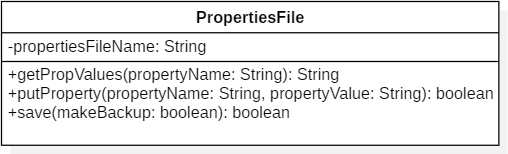
\includegraphics[width=0.4\linewidth]{images/core/classes/PropertiesFile}
\end{figure} 
\subsubsection{Declaration}{
\begin{lstlisting}[frame=none]
public class PropertiesFile
 extends java.lang.Object implements PropertiesFileInterface\end{lstlisting}
\subsubsection{Constructor summary}{
\begin{verse}
\hyperlink{Properties.PropertiesFile()}{{\bf PropertiesFile()}} Default constructor\\
\end{verse}
}
\subsubsection{Method summary}{
\begin{verse}
\hyperlink{Properties.PropertiesFile.getPropValues(java.lang.String)}{{\bf getPropValues(String)}} This Methodes returns the requestet propertie Value\\
\hyperlink{Properties.PropertiesFile.putProperty(java.lang.String, java.lang.String)}{{\bf putProperty(String, String)}} The Method adds a key-value pair to the Properties object.\\
\hyperlink{Properties.PropertiesFile.save(boolean)}{{\bf save(boolean)}} This Method saves the PropertiesFile with the Option to do a Backup of the File\\
\end{verse}
}
\subsubsection{Constructors}{
\vskip -2em
\begin{itemize}
\item{ 
\index{PropertiesFile()}
\hypertarget{Properties.PropertiesFile()}{{\bf  PropertiesFile}\\}
\begin{lstlisting}[frame=none]
public PropertiesFile()\end{lstlisting} %end signature
\begin{itemize}
\item{
{\bf  Description}

Default constructor
}
\end{itemize}
}%end item
\end{itemize}
}
\subsubsection{Methods}{
\vskip -2em
\begin{itemize}
\item{ 
\index{getPropValues(String)}
\hypertarget{Properties.PropertiesFile.getPropValues(java.lang.String)}{{\bf  getPropValues}\\}
\begin{lstlisting}[frame=none]
public java.lang.String getPropValues(java.lang.String propertyName)\end{lstlisting} %end signature
\begin{itemize}
\item{
{\bf  Description}

This Methodes returns the requestet propertie Value
}
\item{
{\bf  Parameters}
  \begin{itemize}
   \item{
\texttt{propertyName} -- propertyName is the name of the Requested Property}
  \end{itemize}
}%end item
\item{{\bf  Returns} -- 
Return the Value to the Requested Property 
}%end item
\end{itemize}
}%end item
\item{ 
\index{putProperty(String, String)}
\hypertarget{Properties.PropertiesFile.putProperty(java.lang.String, java.lang.String)}{{\bf  putProperty}\\}
\begin{lstlisting}[frame=none]
public boolean putProperty(java.lang.String propertyName,java.lang.String propertyValue)\end{lstlisting} %end signature
\begin{itemize}
\item{
{\bf  Description}

The Method adds a key-value pair to the Properties object. To get back to the value later, is called with the key and then return
}
\item{
{\bf  Parameters}
  \begin{itemize}
   \item{
\texttt{propertyName} -- propertyName is the Name of the Property which you want to edit}
   \item{
\texttt{propertyValue} -- propertyValue is the Value of the Property which you want to edit}
  \end{itemize}
}%end item
\item{{\bf  Returns} -- 
true wenn the property got set false otherwise 
}%end item
\end{itemize}
}%end item
\item{ 
\index{save(boolean)}
\hypertarget{Properties.PropertiesFile.save(boolean)}{{\bf  save}\\}
\begin{lstlisting}[frame=none]
public boolean save(boolean makeBackup)\end{lstlisting} %end signature
\begin{itemize}
\item{
{\bf  Description}

This Method saves the PropertiesFile with the Option to do a Backup of the File
}
\item{
{\bf  Parameters}
  \begin{itemize}
   \item{
\texttt{makeBackup} -- true if you want to make a Bachup}
  \end{itemize}
}%end item
\item{{\bf  Returns} -- 
true when the file got saved, false otherwise 
}%end item
\end{itemize}
}%end item
\end{itemize}
}
}
}
